%% -*- Lecture -*-

\synctex=1
\documentclass[11pt]{beamer}
\usepackage{microtype}
\usepackage[utf8]{inputenc}
\usepackage[french]{babel}


\usepackage{lectureb}
\usetheme{CambridgeUS}
\topic{Concurrency}

\begin{document}
\maketitle

\begin{slide}{Review:  Thread package API}
\itms{
  \item \texttt{tid thread\_create (void (*fn) (void *), \rlap{void
          *arg);}}
  \ittms{
    \item Create a new thread that calls \texttt{fn} with \texttt{arg}
  }
  \item \texttt{void thread\_exit ();}
  \item \texttt{void thread\_join (tid thread);}
  \item The execution of multiple threads is interleaved
  \item Can have \emph{\Red{non-preemptive} threads}:
  \ittms{
    \item One thread executes
      exclusively until it makes a blocking call.
  }
  \item Or \emph{\Red{preemptive} threads}:
  \ittms{
    \item May switch to
      another thread between any two instructions.
  }
  \item Using multiple CPUs is inherently preemptive
  \ittms{
    \item Even if you don't take $CPU_0$ away from thread $T$, another
      thread on $CPU_1$ can execute between any two instructions of
      $T$.
  }
%  \item Threads may run simultaneously
%  \ittms{
%    \item E.g., \texttt{create (p1, NULL); create (p2, NULL);}
%    \item \texttt{p1} and \texttt{p2} run interleaved or concurrently
%  }
%  \item Threads have same address space
%  \ittms{
%    \item Usually share some memory locations between threads
%    \item Otherwise, could just have used processes
%  }
%  \item Sharing + Concurrency can lead to unexpected results
}
\end{slide}

\begin{slide}{\hypertarget{prog-a}{Program A}}
\begin{ccode}
  int flag1 = 0, flag2 = 0;

  void p1 (void *ignored) {
    flag1 = 1;
    if (!flag2) { critical_section_1 (); }
  }

  void p2 (void *ignored) {
    flag2 = 1;
    if (!flag1) { critical_section_2 (); }
  }

  int main () {
    tid id = thread_create (p1, NULL);
    p2 (); thread_join (id);
  }
\end{ccode}
\itms{
  \item Can both critical sections run?
}
\end{slide}

\begin{slide}{\hypertarget{prog-b}{Program B}}
\begin{ccode}
  int data = 0, ready = 0;

  void p1 (void *ignored) {
    data = 2000;
    ready = 1;
  }

  void p2 (void *ignored) {
    while (!ready)
      ;
    use (data);
  }

  int main () { ... }
\end{ccode}
\itms{
  \item Can \texttt{use} be called with value 0?
}
\end{slide}

\begin{slide}{Correct answers}
\itms{
  \item Program A:  I don't know
  \item Program B:  I don't know
  \item Why?
  \ittms{
    \item \Red{It depends on your hardware}
    \item If it provides \emph{sequential consistency},
      then answers all No
    \item But not all hardware provides sequential consistency
  }
}
\end{slide}

\begin{slide}{Sequential Consistency}
\begin{itemize}
\item \textit{Sequential consistency}:  The result of execution is as
if all operations were executed in some sequential order, and the
operations of each processor occurred in the order specified by the
program.
\cref{sched/readings/sequential-consistency.pdf}{[Lamport]}
\item Boils down to two requirements:
\begin{enumerate}
  \item Maintaining \textit{program order} on individual processors
  \item Ensuring \textit{write atomicity}
\end{enumerate}
\end{itemize}
\itms{
  \item Without SC, multiple CPUs can be ``worse'' than preemptive
    threads
  \ittms{
    \item May see results that cannot occur with any interleaving on
      \rlap{1 CPU}
  }
  \item Why doesn't all hardware support sequential consistency?
}
\end{slide}

\begin{slide}{SC thwarts hardware optimizations}
\itms{
  \item Can't re-order overlapping write operations
  \ittms{
    \item Coalescing writes to same cache line
  }
  \item Complicates non-blocking reads
  \ittms{
    \item E.g., speculatively prefetch \texttt{data}
    }
  \item Makes cache coherence more expensive
}
\end{slide}

\begin{slide}{SC thwarts compiler optimizations}
\itms{
  \item Code motion
  \item Caching value in register
  \ittms{
    \item Collapse multiple loads/stores of same address into one
      operation
%    \item E.g., \texttt{ready} flag in \hyperlink{prog-b}{Program B}
  }
  \item Common subexpression elimination
  \ittms{
    \item Could cause memory location to be read fewer times
  }
  \item Loop blocking
  \ittms{
    \item Re-arrange loops for better cache performance
  }
  \item Software pipelining
  \ittms{
    \item Move instructions across iterations of a loop to overlap
      instruction latency with branch cost
  }
}
\end{slide}

\begin{slide}{x86 consistency
    [\href{http://www.intel.com/content/dam/www/public/us/en/documents/manuals/64-ia-32-architectures-software-developer-vol-3a-part-1-manual.pdf}{intel
            3a}, \S8.2]}
\itms{
  \item x86 supports multiple consistency/caching models
  \ittms{
    \item Memory Type Range Registers (MTRR) specify consistency for
      ranges of physical memory (e.g., frame buffer)
    \item Page Attribute Table (PAT) allows control for each 4K page
  }
  \item Choices include:
  \ittms{
    \item \textbf{WB}:  Write-back caching (the default)
    \item \textbf{WT}:  Write-through caching (all writes go to
      memory)
    \item \textbf{UC}:  Uncacheable (for device memory)
    \item \textbf{WC}:  Write-combining -- weak consistency \& no
      caching \\
      (used for frame buffers, when sending a lot of data to GPU)
  }
}
\end{slide}


\defverbatim\rdownwr{
\small\openup-.5\jot
\begin{verbatim}
    volatile int flag1 = 0, flag2 = 0;
\end{verbatim}
\begin{verbatim}
    int p1 (void)               int p2 (void)
    {                           {
      register int f, g;          register int f, g;
      flag1 = 1;                  flag2 = 1;
      f = flag1;                  f = flag2;
      g = flag2;                  g = flag1;
      return 2*f + g;             return 2*f + g;
    }                           }
\end{verbatim}}

\begin{frame}
\frametitle{x86 WB consistency}
\smallskip
\itms{
  \item Old x86s (e.g, 486, Pentium 1) had almost SC
  \ittms{
    \item Exception: A read could finish before an earlier write to a
      different location
    \item Which of Programs
      \hyperlink{prog-a}{A},
      \hyperlink{prog-b}{B}, might be affected ?
      \quad \only<2>{\textsl{Just A}}
  }
\pause
  \item Newer x86s also let a CPU read its own writes early
\rdownwr
  \ittms{
    \item E.g., \emph{both} \texttt{p1} and \texttt{p2} can return 2: \\[1ex]
    \item Older CPUs would wait at ``\texttt{f = \ldots}'' until store
      complete
  }
}
\end{frame}

\begin{slide}{x86 atomicity}
\itms{
  \item \texttt{lock} prefix makes a memory instruction atomic
  \ittms{
    \item Usually locks bus for duration of instruction (expensive!)
    \item All lock instructions totally ordered
    \item Other memory instructions cannot be re-ordered w.\ locked
      ones
  }
  \item \texttt{xchg} instruction is always locked (even w/o prefix)
  \item Special fence instructions can prevent re-ordering
  \ittms{
    \item \texttt{mfence} -- can't be reordered w.\ reads or writes
  }

}
\end{slide}

\begin{slide}{Assuming sequential consistency}
\itms{
  \item Important point: \Red{Know your memory model}
  \ittms{
    \item Particularly as OSes typically have their own synchronization
  }
  \item Most application code should avoid depending on memory model
  \ittms{
    \item Obey certain rules, and behavior should be identical to S.C.
  }
  \item Let's for now say we have sequential consistency
  %\item Later will see alpha which doesn't have SC
  \item Example concurrent code: Producer/Consumer
  \ittms{
    \item \texttt{buffer} stores \texttt{BUFFER\_SIZE} items
    \item \texttt{count} is number of used slots
    \item \texttt{out} is next empty buffer slot to fill (if any)
    \item \texttt{in} is oldest filled slot to consume (if any)
  }
}
\end{slide}

\begin{frame}[fragile]
\medskip
\begin{smallccode}
     void producer (void *ignored) {
         for (;;) {
             item *nextProduced = produce_item ();
             while (count == BUFFER_SIZE)
                 /* do nothing */;
             buffer [in] = nextProduced;
             in = (in + 1) % BUFFER_SIZE;
             count++;
         }
     }

     void consumer (void *ignored) {
         for (;;) {
             while (count == 0)
                 /* do nothing */;
             item *nextConsumed =  buffer[out];
             out = (out + 1) % BUFFER_SIZE;
             count--;
             consume_item (nextConsumed);
         }
     }
\end{smallccode}
\itms{
  \item What can go wrong here?
}
\end{frame}

\begin{slide}{Data races}
\itms{
  \item \texttt{count} may have wrong value
  \item Possible implementation of \Blue{\texttt{count++}}
          and \Red{\texttt{count-{}-}}
}
{
\begin{tabular}{@{\qquad\qquad}l@{\qquad}l}
\Blue{register$\gets$count} &
\Red{register$\gets$count} \\
\Blue{register$\gets$register $+$ 1} &
\Red{register$\gets$register $-$ 1} \\
\Blue{count$\gets$register} &
\Red{count$\gets$register} \\
\end{tabular}}
\itms{
  \item Possible execution (count one less than correct):
}
\qquad\qquad \Blue{register$\gets$count} \\
\qquad\qquad \Blue{register$\gets$register $+$ 1} \\
\qquad\qquad \Red{register$\gets$count} \\
\qquad\qquad \Red{register$\gets$register $-$ 1} \\
\qquad\qquad \Blue{count$\gets$register} \\
\qquad\qquad \Red{count$\gets$register} \\
\end{slide}

\begin{slide}{Data races (continued)}
\itms{
  \item What about a single-instruction add?
  \ittms{
    \item E.g., i386 allows single instruction \Blue{\texttt{addl
    \$1,\_count}}
    \item So implement \texttt{count++/-{}-} with one instruction
    \item Now are we safe?
  }
\pause
  \item Not atomic on multiprocessor!
  \ittms{
    \item Will experience exact same race condition
    \item Can potentially make atomic with \texttt{lock} prefix
    \item But \texttt{lock} very expensive
    \item Compiler won't generate it, assumes you don't want penalty
  }
  %\item Note that without SC, even reads can be dangerous
  \item Need solution to \emph{critical section} problem
  \ittms{
    \item Place \texttt{count++} and \texttt{count-{}-} in critical section
    \item Protect critical sections from concurrent execution
  }
}
\end{slide}

\begin{slide}{Desired properties of solution}
\itms{
  \item \emph{Mutual Exclusion}
  \ittms{
    \item Only one thread can be in critical section at a time
  }
  \item \emph{Progress}
  \ittms{
    \item Say no process currently in critical section (C.S.)
    %\item Threads trying to enter C.S. can't be blocked by those not trying
    \item One of the processes trying to enter will eventually get in
  }
  \item \emph{Bounded waiting}
  \ittms{
    \item Once a thread $T$ starts trying to enter the critical
      section, there is a bound on the number of times other threads
      get in
  }
  \item Note progress vs.\ bounded waiting
  \ittms{
    \item If no thread can enter C.S., don't have progress
    \item If thread $A$ waiting to enter C.S. while $B$ repeatedly
      leaves and re-enters C.S. \emph{ad infinitum}, don't have
      bounded waiting
  }
}
\end{slide}

%\begin{slide}{Peterson's solution}
%\itms{
%  \item Still assuming sequential consistency
%  \item Assume two threads, $T_0$ and $T_1$
%  \item Variables
%  \ittms{
%    \item \texttt{int not\_turn;} {\color{comment}-- not this thread's
%      turn to enter C.S.}
%    \item \texttt{bool wants[2];} {\color{comment}-- \texttt{wants[i]}
%      indicates if $T_i$ wants to enter C.S.}
%  }
%  \item Code:
%}
%\begin{ccode}
% for (;;) { /* assume i is thread number (0 or 1) */
%   wants[i] = true;
%   not_turn = i;
%   while (wants[1-i] && not_turn == i)
%     /* other thread wants in and not our turn, so loop */;
%   Critical_section ();
%   wants[i] = false;
%   Remainder_section ();
% }
%\end{ccode}
%\end{slide}
%
%\begin{slide}{Does Peterson's solution work?}
%\begin{smallccode}
%      for (;;) { /* code in thread i */
%        wants[i] = true;
%        not_turn = i;
%        while (wants[1-i] && not_turn == i)
%          /* other thread wants in and not our turn, so loop */;
%        Critical_section ();
%        wants[i] = false;
%        Remainder_section ();
%      }
%\end{smallccode}
%\itms{
%  \item Mutual exclusion -- can't both be in C.S.
%  \ittms{
%    \item Would mean \texttt{wants[0] == wants[1] == true}, \\
%          so \texttt{not\_turn} would have blocked one thread from C.S.
%  }
%  \item Progress -- If $T_{1-i}$ not in C.S., can't block $T_i$
%  \ittms{
%    \item Means \texttt{wants[1-i] == false}, so $T_i$ won't loop
%  }
%  \item Bounded waiting -- similar argument to progress
%  \ittms{
%    \item If $T_i$ wants lock and $T_{1-i}$ tries to re-enter,
%      $T_{1-i}$ will set \\
%      \texttt{not\_turn = 1 - i}, allowing $T_i$ in
%  }
%}
%\end{slide}

\begin{slide}{Mutexes}
\itms{
  \item Must adapt to machine memory model if not S.C.
  \ittms{
    \item Ideally want your code to run everywhere
  }
  \item Want to insulate programmer from implementing synchronization
    primitives
  \item Thread packages typically provide \emph{mutexes}: \\
    \texttt{void mutex\_init (mutex\_t *m, \ldots);} \\
    \texttt{void mutex\_lock (mutex\_t *m);} \\
    \texttt{int mutex\_trylock (mutex\_t *m);} \\
    \texttt{void mutex\_unlock (mutex\_t *m);} \\
  \ittms{
    \item Only one thread acquires \texttt{m} at a time, others wait
  }
}
\end{slide}

\begin{slide}{Thread API contract}
\itms{
  \item \Red{All global data should be protected by a mutex!}
  \ittms{
    \item Global = accessed by more than one thread, at least one
      write
    \item Exception is initialization, before exposed to
      other threads
    \item This is the responsibility of the application writer
  }
  \item If you use mutexes properly, behavior should be
    indistinguishable from Sequential Consistency
  \ittms{
    \item This is the responsibility of the threads package (\&
      compiler)
    \item Mutex is broken if you use properly and don't see S.C.
  }
  \item OS kernels also need synchronization
  \ittms{
    \item May or may not look like mutexes
  }
}
\end{slide}

\begin{slide}{Same concept, many names}
\itms{
  \item Most popular application-level thread API:  \emph{pthreads}
  \ittms{
    \item Function names in this lecture all based on \emph{pthreads}
    \item Just add \texttt{pthread\_} prefix
    \item E.g., \texttt{pthread\_mutex\_t},
      \texttt{pthread\_mutex\_lock}, \ldots
  }
}
\end{slide}


\begin{slide}{Improved producer}
\begin{ccode}[classoffset=2,morekeywords={mutex_lock,mutex_unlock},keywordstyle=\color{red}]
mutex_t mutex = MUTEX_INITIALIZER;

void producer (void *ignored) {
    for (;;) {
        item *nextProduced = produce_item ();

        mutex_lock (&mutex);
        while (count == BUFFER_SIZE) {
          mutex_unlock (&mutex);  /* <--- Why? */
          thread_yield ();
          mutex_lock (&mutex);
        }

        buffer [in] = nextProduced;
        in = (in + 1) % BUFFER_SIZE;
        count++;
        mutex_unlock (&mutex);
    }
}
\end{ccode}
\end{slide}

\begin{slide}{Improved consumer}
\begin{ccode}[classoffset=2,morekeywords={mutex_lock,mutex_unlock},keywordstyle=\color{red}]
void consumer (void *ignored) {
    for (;;) {
        mutex_lock (&mutex);
        while (count == 0) {
          mutex_unlock (&mutex);
          thread_yield ();
          mutex_lock (&mutex);
        }

        item *nextConsumed =  buffer[out];
        out = (out + 1) % BUFFER_SIZE;
        count--;
        mutex_unlock (&mutex);

        consume_item (nextConsumed);
    }
}
\end{ccode}
\end{slide}

\begin{slide}{Condition variables}
\itms{
  \item Busy-waiting in application is a bad idea
  \ittms{
    \item Thread consumes CPU even when can't make progress
    \item Unnecessarily slows other threads and processes
  }
  \item Better to inform scheduler of which threads can run
  \item Typically done with \emph{condition variables}
  \item \texttt{void cond\_init (cond\_t *, \ldots);}
  \ittms{
    \item Initialize
  }
  \item \texttt{void cond\_wait (cond\_t *c, mutex\_t *m);}
  \ittms{
    \item Atomically unlock \texttt{m} and sleep until \texttt{c} signaled
    \item Then re-acquire \texttt{m} and resume executing
  }
  \item \texttt{void cond\_signal (cond\_t *c);} \\
        \texttt{void cond\_broadcast (cond\_t *c);}
  \ittms{
    \item Wake one/all threads waiting on \texttt{c}
  }
}
\end{slide}

\begin{slide}{Improved producer}
\begin{ccode}[classoffset=2,morekeywords={cond_wait,cond_signal},keywordstyle=\color{red}]
mutex_t mutex = MUTEX_INITIALIZER;
cond_t nonempty = COND_INITIALIZER;
cond_t nonfull = COND_INITIALIZER;

void producer (void *ignored) {
    for (;;) {
        item *nextProduced = produce_item ();

        mutex_lock (&mutex);
        while (count == BUFFER_SIZE)
          cond_wait (&nonfull, &mutex);

        buffer [in] = nextProduced;
        in = (in + 1) % BUFFER_SIZE;
        count++;
        cond_signal (&nonempty);
        mutex_unlock (&mutex);
    }
}
\end{ccode}
\end{slide}

\begin{slide}{Improved consumer}
\begin{ccode}[classoffset=2,morekeywords={cond_wait,cond_signal},keywordstyle=\color{red}]
void consumer (void *ignored) {
    for (;;) {
        mutex_lock (&mutex);
        while (count == 0)
          cond_wait (&nonempty, &mutex);

        item *nextConsumed =  buffer[out];
        out = (out + 1) % BUFFER_SIZE;
        count--;
        cond_signal (&nonfull);
        mutex_unlock (&mutex);

        consume_item (nextConsumed);
    }
}
\end{ccode}
\end{slide}

\begin{slide}{Re-check conditions}
\itms{
  \item Always re-check condition on wake-up:
}
\vspace*{-.5\baselineskip}
\begin{ccode}
        `\Red{while}' (count == 0)  /* not `\Red{if}' */
          cond_wait (&nonempty, &mutex);
\end{ccode}
\itms{
  \item Otherwise, breaks with two consumers
  \begin{itemize}
    \item Start with empty buffer, then:
  \end{itemize}
}
{\small\openup-1\jot
\halign{#\hfil \quad & \quad #\hfil \quad & \quad # \hfil \cr
\hfil \vrule width0pt depth 8pt{}$C_1$ & \hfil $C_2$ & $P$ \cr
\texttt{cond\_wait (\ldots);} & & {\texttt{mutex\_lock (\ldots);}}\cr
& & \hfil $\vdots$ \cr
& & \texttt{count++;} \cr
& & \texttt{cond\_signal (\ldots);} \cr
& {\texttt{mutex\_lock (\ldots);}} & \texttt{mutex\_unlock (\ldots);} \cr
& \texttt{if (count == 0)} & \cr
& \hfil $\vdots$ & \cr
& \emph{use} \texttt{buffer[out]} \ldots & \cr
& \texttt{count--;} & \cr
& \texttt{mutex\_unlock (\ldots);} & \cr
\noalign{\smallskip}
\multispan{3}
\emph{use} \texttt{buffer[out]} \ldots
    \Red{$\;\;\longleftarrow$ No items in buffer}\hfil\cr
%\texttt{\Red{count-{}-};} & & \cr
}}
\end{slide}


\defverbatim\condwomutex{
\begin{ccode}
             while (count == BUFFER_SIZE) {
               mutex_unlock (&mutex);
               cond_wait (&nonfull);
               mutex_lock (&mutex);
             }
\end{ccode}}

\defverbatim[colored]\condwomutexbug{
\small\openup-.17\baselineskip
{\color{comment}
\begin{verbatim}
   PRODUCER                        CONSUMER
\end{verbatim}
}
\begin{verbatim}
   while (count == BUFFER_SIZE)
     mutex_unlock (&mutex);
                                   mutex_lock (&mutex);
                                   ...
                                   count--;
                                   cond_signal (&nonfull);
     cond_wait (&nonfull);
\end{verbatim}
}

\begin{slide}{Condition variables (continued)}
\itms{
  \item Why must \texttt{cond\_wait} both release mutex \& sleep?
  \item Why not separate mutexes and condition variables?
}
\condwomutex
\begin{overprint}
\onslide<2->{
\itms{
  \item Can end up stuck waiting when bad interleaving
}
\condwomutexbug
}
\end{overprint}
\end{slide}



\begin{slide}{Semaphores
    \href{http://www.cs.utexas.edu/users/EWD/transcriptions/EWD01xx/EWD123.html}{[Dijkstra]}}
\itms{
  \item A \emph{Semaphore} is initialized with an integer $N$
  \item Provides two functions:
  \ittms{
    \item \texttt{sem\_wait (S)}\quad  (originally called $P$)
    \item \texttt{sem\_signal (S)}\quad (originally called $V$)
  }
  \item Guarantees \texttt{sem\_wait} will return only $N$ more times than
    \texttt{sem\_signal} called
  \ittms{
    \item Example:  If $N==1$, then semaphore is a mutex with
      \texttt{sem\_wait} as lock and \texttt{sem\_signal} as unlock
  }
  \item Semaphores give elegant solutions to some problems
  \item Linux primarily uses semaphores for sleeping locks
  \ittms{
    \item \texttt{sema\_init}, \texttt{down\_interruptible},
      \texttt{up}, \ldots
%\item Also weird reader-writer semaphores, \texttt{rw\_semaphore}
%  \href{http://www.linuxjournal.com/article/5833}{[Love]}
% Seems abstractions called "lock" in the linux kernel are all
% spinlocks.  So they are using semaphores as sleeping locks.
    \item But evidence might favor
      mutexes~\href{http://www.kernel.org/doc/Documentation/mutex-design.txt}{[Molnar]}
  }
}
\end{slide}

\begin{frame}[fragile]
\frametitle{Semaphore producer/consumer}
\itms{
  \item Initialize \texttt{nonempty} to 0 (block consumer when buffer empty)
  \item Initialize \texttt{nonfull} to $N$ (block producer when queue full)
}
\begin{smallccode}[classoffset=2,morekeywords={sem_wait,sem_signal},keywordstyle=\color{red}]
     void producer (void *ignored) {
         for (;;) {
             item *nextProduced = produce_item ();
             sem_wait (&nonfull);
             buffer [in] = nextProduced;
             in = (in + 1) % BUFFER_SIZE;
             sem_signal (&nonempty);
         }
     }
     void consumer (void *ignored) {
         for (;;) {
             sem_wait (&nonempty);
             item *nextConsumed =  buffer[out];
             out = (out + 1) % BUFFER_SIZE;
             sem_signal (&nonfull);
             consume_item (nextConsumed);
         }
     }
\end{smallccode}
\end{frame}


\begin{slide}{Other thread package features}
\itms{
  \item Alerts -- cause exception in a thread
  %\item Trylock -- don't block if can't acquire mutex
  \item Timedwait -- timeout on condition variable
  \item Shared locks -- concurrent read accesses to data
  \item Thread priorities -- control scheduling policy
  \ittms{
    \item Mutex attributes allow various forms of \emph{priority
        donation} \\
      (will be familiar concept after lab 1)
  }
  \item Thread Local Storage
}
\end{slide}

\defverbatim[colored]\muteximp{
\begin{smallccode}[classoffset=2,morekeywords={lower_level_lock_t,lk},
        keywordstyle=\color{red}]
    typedef struct mutex {
      bool is_locked;            /* true if locked */
      thread_id_t owner;         /* thread holding lock, if locked */
      thread_list_t waiters;     /* threads waiting for lock */

      lower_level_lock_t lk;     /* Protect above fields */
    };
\end{smallccode}
}

\begin{frame}
\frametitle{Implementing synchronization}
\itms{
  \item User-visible mutex is straight-forward data structure
\muteximp
  \item Need lower-level lock \texttt{lk} for mutual exclusion
  \ittms{
    \item Internally, \texttt{mutex\_*} functions bracket code with \\
\texttt{lock(mutex->lk)} \ldots\ \texttt{unlock(mutex->lk)}
    \item Otherwise, data races!
    (E.g., two threads manipulating \texttt{waiters})
  }
  \item \Red{How to implement \texttt{lower\_level\_lock\_t}?}
  \ittms{
    \item Use hardware support for synchronization
  }
}
\end{frame}

\begin{slide}{Approach \#1: Disable interrupts}
\itms{
  \item Only for apps with $n:1$ threads (1 kthread)
  \ittms{
    \item Cannot take advantage of multiprocessors
    \item But sometimes most efficient solution for uniprocessors
  }
  \item \hypertarget{DNI}Have per-thread ``do not interrupt'' (DNI) bit
  \item \texttt{lock (lk)}: sets thread's DNI bit
  \item If timer interrupt arrives
  \ittms{
    \item Check interrupted thread's DNI bit
    \item If DNI clear, preempt current thread
    \item If DNI set, set ``interrupted'' (I) bit \& resume current
      thread
  }
  \item \texttt{unlock (lk)}: clears DNI bit \emph{and} checks I bit
  \ittms{
    \item If I bit is set, immediately yields the CPU
  }
}
\end{slide}

\defverbatim\spinlock{
\begin{ccode}
     #define lock(lockp)    while (test_and_set (lockp))
     #define trylock(lockp) (test_and_set (lockp) == 0)
     #define unlock(lockp)  *lockp = 0
\end{ccode}}

\begin{frame}
\frametitle{Approach \#2: Spinlocks}
\itms{
  \item Most CPUs support atomic read-[modify-]write
  %\item Most CPUs have atomic read-write or atomic read-modify-write
  \item Example:  \texttt{int test\_and\_set (int *lockp);}
  \ittms{
    \item Atomically sets \texttt{*lockp = 1} and returns old value
    \item Special instruction -- can't be implemented in portable C
    }
  \item Use this instruction to implement \emph{spinlocks}:
\spinlock
  \item Spinlocks implement mutex's \texttt{lower\_level\_lock\_t}
  \item Can you use spinlocks instead of mutexes?
  \ittms{
    \item Wastes CPU, especially if thread holding lock not running
    \item Mutex functions have short C.S., less likely to be preempted
    \item On multiprocessor, sometimes good to spin for a bit, then yield
  }
%  \item But gratuitous context switch has cost
%  \ittms{
%    \item On MP, sometimes good to spin for a bit, then yield
%  }
}
\end{frame}

%\begin{slide}{Synchronization on x86}
%\itms{
%  \item Test-and-set only one possible atomic instruction
%  \item x86 \texttt{xchg} instruction, exchanges reg with mem
%  \ittms{
%    \item Can use to implement test-and-set
%  }
%}
%\begin{asm}
%        _test_and_set:
%                movl    8(%esp), %edx   # %edx = lockp
%                movl    $1, %eax        # %eax = 1
%                xchgl   %eax, (%edx)    # swap (%eax, *lockp)
%                ret
%\end{asm}%$
%\itms{
%  \item CPU locks memory system around read and write
%  \ittms{
%    \item Recall \texttt{xchgl} always acts like it has \texttt{lock} prefix
%    \item Prevents other uses of the bus (e.g., DMA)
%  }
%  \item Usually runs at memory bus speed, not CPU speed
%  \ittms{
%    \item Much slower than cached read/buffered write
%  }
%}
%\end{slide}

\defverbatim[colored]\splhigh{
\begin{ccode}
    int x = splhigh ();   /* Disable interrupts */
    /* touch data shared with interrupt handler ... */
    splx (x);             /* Restore previous state */
\end{ccode}
}

%\begin{frame}
%\frametitle{Kernel Synchronization}
%\itms{
%  \item \Red{Should kernel use locks or disable interrupts?}
%  \item Old UNIX had non-preemptive threads, no mutexes
%  \ittms{
%    \item Interface designed for single CPU, so \texttt{count++} etc.\ not data race
%    \item
%    \ldots\emph{Unless} memory shared with an interrupt handler
%    \\[1ex]
%    \splhigh
%    \item C.f.,
%      \cref{pintos/pintos_6.html\#SEC101}{Pintos}
%      \texttt{intr\_disable} / \texttt{intr\_set\_level}
%  }
%  \item Used arbitrary pointers like condition variables
%  \ittms{
%    \item \texttt{int [t]sleep (void *ident, int priority, ...);} \\
%      put thread to sleep; will wake up at \texttt{priority}
%      ($\sim$\texttt{cond\_wait})
%    \item \texttt{int wakeup (void *ident);} \\
%      wake up all threads sleeping on \texttt{ident}
%      ($\sim$\texttt{cond\_broadcast})
%  }
%}
%\end{frame}

%\begin{slide}{Kernel locks}
%\itms{
%  \item Nowadays, should design for multiprocessors
%  \ittms{
%    \item Even if first version of OS is for uniprocessor
%    \item Someday may want multiple CPUs and need \emph{preemptive}
%      threads
%    \item That's why Pintos uses locks
%  }
%  \item Multiprocessor performance needs fine-grained locks
%  \ittms{
%    \item Want to be able to call into the kernel on multiple CPUs
%  }
%  \item \Red{If kernel has locks, should it ever disable interrupts?}
%\pause
%  \ittms{
%    \item Yes!  Can't sleep in interrupt handler, so can't wait for lock
%    \item So even modern OSes have support for disabling interrupts
%    \item Often uses \hyperlink{DNI}{DNI} trick, which is cheaper than masking
%      interrupts in hardware
%  }
%}
%\end{slide}

%% \begin{slide}{UNIX Synchronization 2}
%% \itms{
%%   \item Need to relinquish CPU when waiting for events
%%   \ittms{
%%     \item Disk read, network packet arrival, pipe write, signal, etc.
%%   }
%%   \item \texttt{int tsleep(void *ident, int priority, ...);}
%%   \ittms{
%%     \item Switches to another process
%%     \item \texttt{ident} is arbitrary pointer---e.g., buffer address
%%     \item \texttt{priority} is priority at which to run when woken up
%%     \item \textsc{PCATCH}, if ORed into \texttt{priority}, means wake
%%           up on signal
%%     \item Returns 0 if awakened, or \textsc{ERESTART}/\textsc{EINTR} on
%%           signal
%%   }
%%   \item \texttt{int wakeup(void *ident);}
%%   \ittms{
%%     \item Awakens all processes sleeping on \texttt{ident}
%%     \item Restores SPL to value when they went to sleep \\
%%       (so fine to sleep at splhigh)
%%   }
%% }
%% \end{slide}


%% \begin{slide}{Monitors
%%     [BH]\cref{sched/readings/monitors.pdf}{[Hoar]}}
%% \itms{
%%   \item Programming language construct
%%   \ittms{
%%     \item Possibly less error prone than raw mutexes, but less flexible too
%%     \item Basically a class where only one procedure executes at a time
%%   }
%% }
%% \begin{ccode}
%%           monitor monitor-name
%%           {
%%             // shared variable declarations
%%             procedure P1 (...) { ... }
%%             ...
%%             procedure Pn (...) { ... }

%%             Initialization code (..) { ... }
%%           }
%% \end{ccode}
%% \itms{
%%   \item Can implement mutex w.\ monitor or vice versa
%%   \ittms{
%%     \item But monitor alone doesn't give you condition variables
%%     \item Need some other way to interact w.\ scheduler
%%     \item Use \emph{conditions}, which are essentially condition variables
%%   }
%% }
%% \end{slide}

%% \begin{slide}{Monitor implementation}
%% \centerline{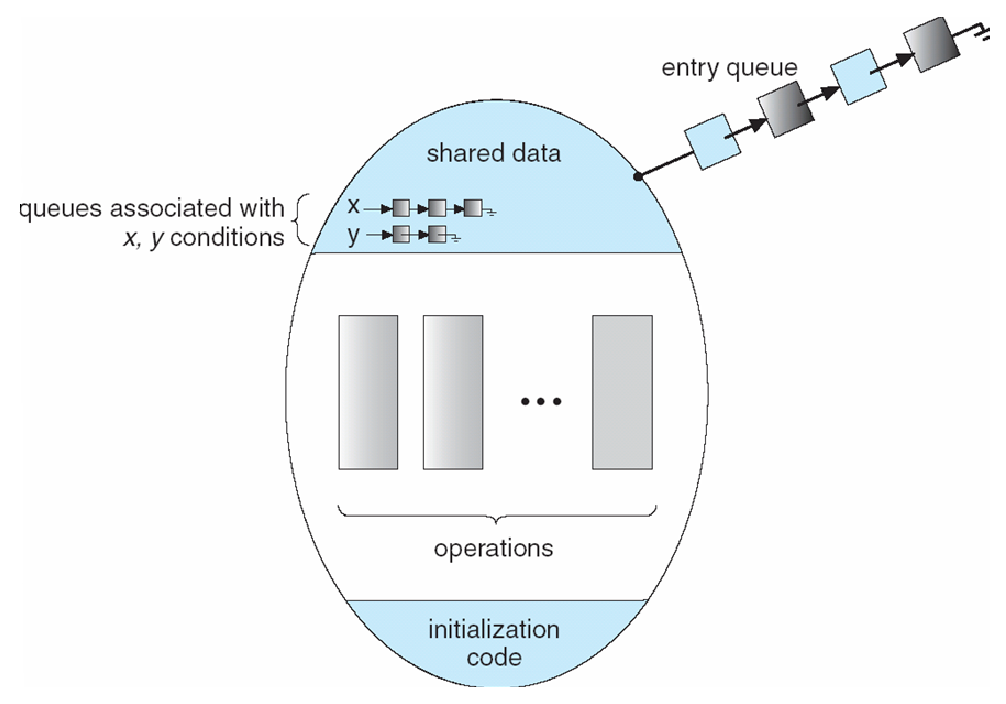
\includegraphics[height=2.2in]{figs/monitorcond}}
%% \medskip
%% \itms{
%%   \item Queue of threads waiting to get in
%%   \ittms{
%%     \item Might be protected by spinlock
%%   }
%%   \item Queues associated with conditions
%% }
%% \end{slide}
\end{document}

\begin{slide}{Readers-Writers Problem}
\itms{
  \item Multiple threads may access data
  \ittms{
    \item \emph{Readers} -- will only observe, not modify data
    \item \emph{Writers} -- will change the data
  }
  \item Goal: allow multiple readers or one single writer
  \ittms{
    \item Thus, lock can be \emph{shared} amongst concurrent readers
  }
  \item Can implement with other primitives
  \ittms{
    \item Keep integer \texttt{i} -- \# or readers or -1 if held by writer
  }
}
\end{slide}

\begin{slide}{Implementing shared locks}
\vspace*{-2ex}
\begin{myverb}
struct sharedlk {
  int i;
  mutex_t m;
  cond_t c;
};

void AcquireExclusive (sharedlk *sl) {
  lock (sl->m);
  while (sl->i) { wait (sl->m, sl->c); }
  sl->i = -1;
  unlock (sl->m);
}

void AcquireShared (sharedlk *sl) {
  lock (sl->m);
  while (sl->i < 0) { wait (sl->m, sl->c); }
  sl->i++;
  unlock (sl->m);
}
\end{myverb}
\end{slide}

\begin{slide}{shared locks (continued)}
\begin{myverb}
void ReleaseShared (sharedlk *sl) {
  lock (sl->m);
  if (!--sl->i) signal (sl->c);
  unlock (sl->m);
}

void ReleaseExclusive (sharedlk *sl) {
  lock (sl->m);
  sl->i = 0;
  broadcast (sl->c);
  unlock (sl->m);
}
\end{myverb}
\itms{
  \item Note:  Must deal with starvation
}
\end{slide}

\end{document}



\begin{slide}{Benign races}
\itms{
  \item Sometimes ``cheating'' buys efficiency\ldots
  \item Care more about speed than accuracy
}
\begin{myverb}
    hits++;  // each time someone accesses web site
\end{myverb}
\itms{
  \item Know you can get away with race
}
\begin{myverb}
    if (!initialized) {
      lock (m);
      if (!initialized) { initialize (); initialized = 1; }
      unlock (m);
    }
\end{myverb}
\end{slide}

\begin{slide}{Detecting data races}
\itms{
  \item Static methods (hard)
  \item Debugging painful---race might occur rarely
  \item Instrumentation---modify program to trap memory accesses
  \item Lockset algorithm (eraser) particularly effective:
  \ittms{
    \item For each global memory location, keep a ``lockset''
    \item On each access, remove any locks not currently held
    \item If lockset becomes empty, abort:  No mutex protects data
    \item Catches potential races even if they don't occur
  }
}
\end{slide}



\end{document}
